\documentclass[a4paper]{article}
\author{Kevin A. Blondino \\
	\texttt{Supervisor: dr. H.J. de Blank}}
\title{Radial Electric Field-Generating Terms in L-H Transitions}
\date{\today}

%{{{ Packages
\usepackage{fullpage,amsmath,natbib,graphicx,indentfirst}

\usepackage{lipsum}

\usepackage{xcolor}
\newcommand\mynotes[1]{\textcolor{red}{#1}}

\linespread{1.05}
%}}}

%{{{ Two Figures Side-by-Side
\newsavebox\IBoxA \newsavebox\IBoxB \newlength\IHeight
\newcommand\TwoFig[6]{% Image1 Caption1 Label1 Im2 Cap2 Lab2
	\sbox\IBoxA{\includegraphics[width=0.45\textwidth]{#1}}
	\sbox\IBoxB{\includegraphics[width=0.45\textwidth]{#4}}%
	\ifdim\ht\IBoxA>\ht\IBoxB
		\setlength\IHeight{\ht\IBoxB}%
	\else\setlength\IHeight{\ht\IBoxA}\fi
	\begin{figure}[!htb]
	\minipage[t]{0.45\textwidth}\centering
	\includegraphics[height=\IHeight]{#1}
	\caption{#2}\label{#3}
	\endminipage\hfill
	\minipage[t]{0.45\textwidth}\centering
	\includegraphics[height=\IHeight]{#4}
	\caption{#5}\label{#6}
	\endminipage
	\end{figure}%
}
%}}}

%--------------------------------------

\begin{document}
\maketitle

%--------------------------------------

%{{{ Abstract
\begin{abstract}
	From the discovery of H-mode by ASDEX in 1982, inquiry in the mechanisms that cause the transition from L-mode have become a topic of interest.
	This transition is a bifurcation in the anomalous transport just inside the separatrix in a divertor tokamak.
	A key mechanism is the generation of a large radial electric field and corresponding $\mathbf{E}\times\mathbf{B}$ flow and flow shear near the edge.

	This radial electric field at the edge can be found by investigating the nonambipolar fluxes. Using a set of nonlinear partial differential equations with boundary conditions, the dominance of field-generating effect can be determined for a particular set of tokamak parameters.
\end{abstract}
%}}}

\section{Introduction and Background}
\subsection{Transition}
In 1982, a new NBI system was install in the ASDEX tokamak, which pushed into a new realm.
A new level of energy confinement time was achieved, typically a factor of 2 or more than previous.
This state of operation was coined the high-confinement (H-) mode, and is considered necessary for the future of nuclear fusion as an energy source \cite{wagner_development_1984}.
%\begin{figure}
%	\centering
%\begin{minipage}{0.48\linewidth}
%	\centering
%	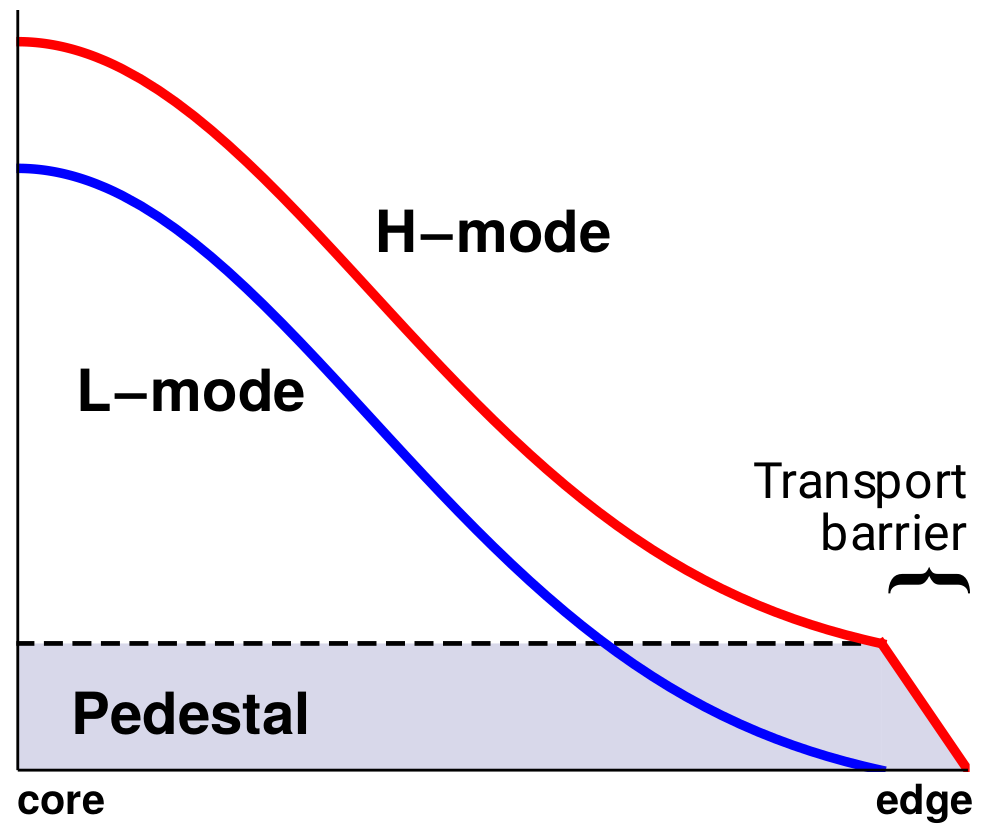
\includegraphics[width=0.8\textwidth]{../Graphics/L-mode_H-mode_compare.png}
%	\caption{A comparison of the radial pressure profiles of L-mode and H-mode \cite{weymiens_bifurcation_2014}.}
%	\label{fig:L-mode_H-mode_compare}
%\end{minipage}
%\hfill
%\begin{minipage}{0.48\linewidth}
%	\centering
%	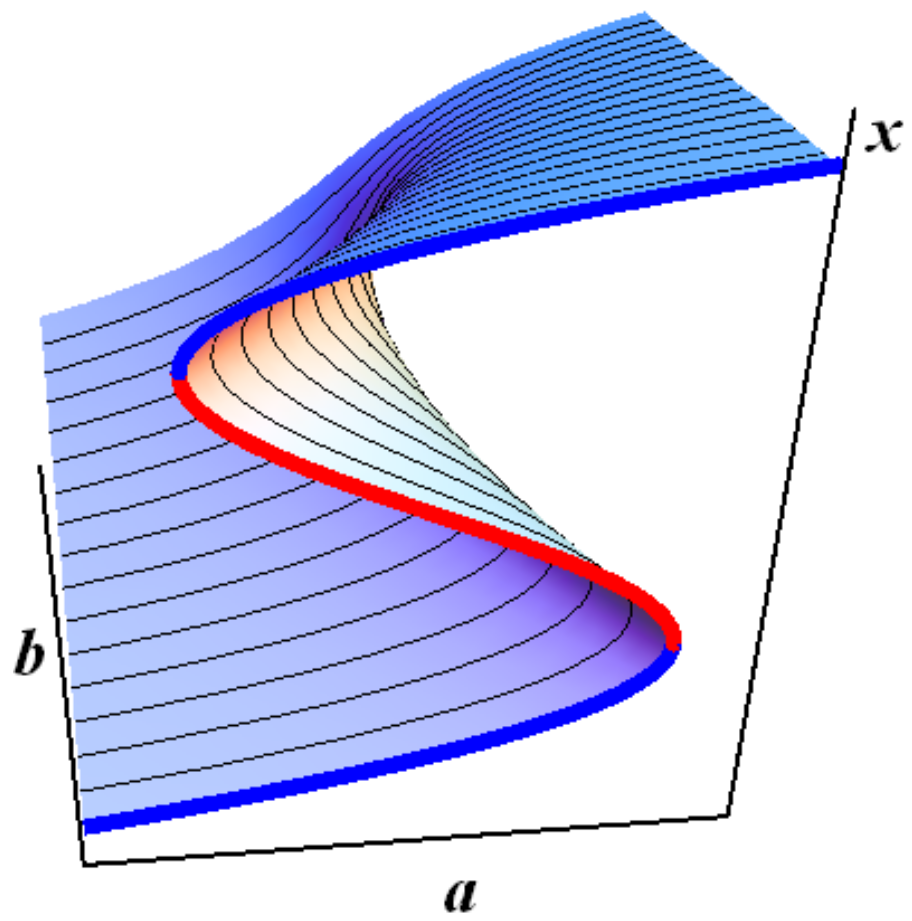
\includegraphics[width=0.8\textwidth]{../Graphics/Bif_3D.png}
%	\caption{The bifurcation in parameter space. The parameter $b$ dictates the size of the hysteresis, until the two fold bifurcations merge into a cusp \cite{weymiens_bifurcation_2014}.}
%	\label{fig:Bif_3D}
%\end{minipage}
%\end{figure}

The transport of particles and energy has been discovered to be dominated by anomalous transport, which is generally assumed to be generated by turbulence driven by micro-instabilities \cite{freidberg_plasma_2007}.
The transition between low-confinement (L-) mode and H-mode is a bifurcation in the turbulent transport at the edge of the tokamak in a divertor setup.

Interestingly, the universal bifurcation behavior includes hysteresis between the L-H and H-L transitions in so-called sharp transitions, ones most commonly observed.
In the context of this transition, the plasma will go into H-mode once a certain heating threshold is surpassed.
However, the plasma will go back to L-mode once the heating power is reduced below a lower threshold, allowing for non-unique solutions of the plasma state.
For lower-density operations, the plasma will not exhibit hysteresis, and transitions are smooth.
In addition, a third type have been observed in which the state will rapidly oscillate between the two modes \cite{weymiens_bifurcation_2014}.

\TwoFig{../Graphics/L-mode_H-mode_compare.png}
	{A comparison of the radial pressure profiles of L-mode and H-mode \cite{weymiens_bifurcation_2014}.}
	{fig:L-mode_H-mode_compare}
	{../Graphics/Bif_3D.png}
	{The bifurcation in parameter space. The parameter $b$ dictates the size of the hysteresis, until the two fold bifurcations merge into a cusp \cite{weymiens_bifurcation_2014}.}
	{fig:Bif_3D}

\subsection{Electric Field}
A key mechanism for the transition is the suppresion of this transport by the generation of a large radial electric field and the corresponding $\mathbf{E}\times\mathbf{B}$ flows and large flow shear near the edge.
A plethora of individual mechanisms for the generation of such an electric field have been proposed, most of which can be viewed as separate contributions in a radial Poisson's law.

The radial electric field $E_r$ is deduced from the radial force balance for any plasma species $j$, as follows:
\begin{equation}
	E_r \,=\, -\frac{1}{n_j e_j} \frac{\text{d} p_j}{\text{d} r} + V_{\theta j} B_\phi - V_{\phi j} B_\theta
	\label{eq:E_r}
\end{equation}
In the above, $e_j$ represents the charge of the $j$-th species, $n_j$ is the density, $p_j$ is the pressure, and $V_{\theta j}$ and $V_{\phi j}$ are the poloidal and toroidal velocities, respectively.
This grants changes in the radial electric field to be associated with changes in radial gradient of the pressure or either velocities \cite{connor_review_2000}\cite{staps_backstepping_2017}.
However, determining these values is difficult due to large possible error in experiment.

A more practical approach in finding the field utilizes knowledge of the particle fluxes.
These fluxes that affect the plasma momentum can be classified into ambipolar and nonambipolar.
Ambipolar fluxes are equal for ions and electrons, and contribute zero radial current.
Nonambipolar fluxes violate the ambipolarity constraint, which causes the radial electric field to generate a return current such that the divergence of the plasma current vanishes.
These fluxes therefore depend on the radial electric field \cite{callen_toroidal_2009}.
%\begin{equation}
%	\langle \mathbf{J}\cdot\nabla p\rangle \,=\, \sum_s q_s \Gamma_s^\text{na} \,=\, 0
%	\label{eq:ambipolar_constraint}
%\end{equation}

\subsection{Transition Model}
The basic model for the transition, developed first by Itoh et al. \cite{itoh_edge_1991} and later expanded by Zohm \cite{zohm_dynamic_1994}, contains the continuity equations of energy and density to describe H-mode.
The generation of a transport barrier could then be caused by a local reduction of the transport coeffecients.
Such a model was further adapted by Weymiens \cite{weymiens_bifurcation_2014} into the following form.
\begin{equation}
	\epsilon \frac{\partial Z}{\partial t} \,=\, \mu \frac{\partial^2 Z}{\partial x^2} + \frac{c_n T}{n^2} \frac{\partial n}{\partial x} + \frac{c_T}{n} \frac{\partial T}{\partial x} + G(Z)
	\label{eq:pde}
\end{equation}
This model uses $Z$, the radial electric field normalized with respect to the ion Larmor (gyro-)radius $\rho_{\theta i}$ and temperature $T$.
\begin{equation}
	Z \,=\, \frac{\rho_{\theta i} e E_r}{T}, ~~~~~ \rho_{\theta i} \,=\, \frac{m_i v_{\phi i}}{e B_\theta}
	\label{eq:normalization}
\end{equation}
% Another way to look at this equation is that the term on the left is the polarization radial current, the 2nd-derivative is due to shear viscosity.
The left-hand side of Eq.~\ref{eq:pde} describes the radial current due to polarization, with $\epsilon = B_\theta^2 / (B^2 \nu_i)$, the dielectric constant.
The 2nd-derivative term describes the radial current due to the anomalous shear viscosity of the $\mathbf{E}\times\mathbf{B}$ drift, with $\mu$ as the ratio of viscosity to collisition frequency.
The 1st-derivative terms are due to all ambipolar cross-field fluxes.
$G(Z)$ is a cubic polynomial that approximates the remaining electric field-inducing contributions.
It has an inflection point at in $Z$-space at $Z_S$ and coefficients $a$, $b$, and $c$:
\begin{equation}
	G(Z) \,=\, a + b(Z - Z_S) + c(Z - Z_S)^3
\end{equation}


%--------------------------------------

\section{Problem Statement}
Although there has been compilations of different theories describing the transition, there is yet to be a conclusive, comprehensive one \cite{connor_review_2000}.
This specifically applies to the overall dependence of each effect on the radial electric field.
Therefore, the problem can be stated simply: \textbf{Which electric field-generating terms are dominant in concrete experimental tokamak conditions?}

%--------------------------------------

\section{Project Plan}
The months of May through July have included extensive literature study.
By the end of August, my hope is to have a mathematical model working in which I start to obtain preliminary results.
September through October will include running through the calculations to obtain and parse through data, and subsequent comparison with published data.

%--------------------------------------

%{{{ References
%\newpage
\bibliographystyle{plain}
%\nocite{*}
\bibliography{../References/References}
%}}}
\end{document}
